\chapter{First step}
\label{intro}


First, download and install the {\TeX}/{\LaTeX} distribution:
\begin{itemize}
\item MiKTeX (\url{https://miktex.org/})
\item Tex live(\url{https://www.tug.org/texlive/})
\item MacTeX (\url{https://www.tug.org/mactex/}), Mac OS only.
\end{itemize}

Although those {\TeX}/{\LaTeX} distributions all include a {\LaTeX} editor, I prefer use Texmaker(\url{http://www.xm1math.net/texmaker/}) or TeXstudio (\url{https://www.texstudio.org/}).

Then, we can create a document in {\LaTeX}.

\begin{lstlisting}[language=Tex]
\documentclass{article}
\begin{document}
This is hello {\LaTeX} !.
\end{document}
\end{lstlisting}

Save those code into a file with the extension \notecolor{.tex}, e.g., helloworld.tex. and open it with Texmaker.
Follow the steps shown in Figure \ref{fig.latex}, we can obtain the result .pdf file.
First, we use {\LaTeX} to compile this .tex file to generate a .dvi file.
Next, we use \notecolor{DVI$->$PDF} to convert .dvi to .pdf file.
Or, we can use PDFLaTeX to generate the pdf file directly as depicted in Figure \ref{fig.pdflatex}.
Then, we can view the pdf file by the built-in viewer.


\begin{figure*}[!t]
\centering
\subfloat[LaTeX]{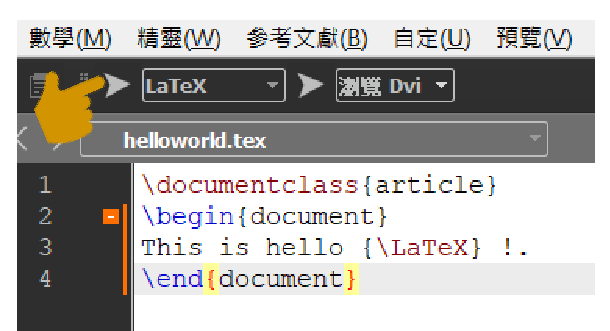
\includegraphics[width= 2.3in]{figs//s1}}
\subfloat[DVI to PDF]{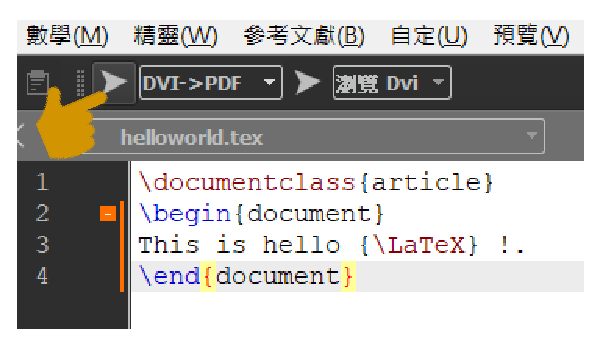
\includegraphics[width= 2.3in]{figs//s2}}
\subfloat[View PDF]{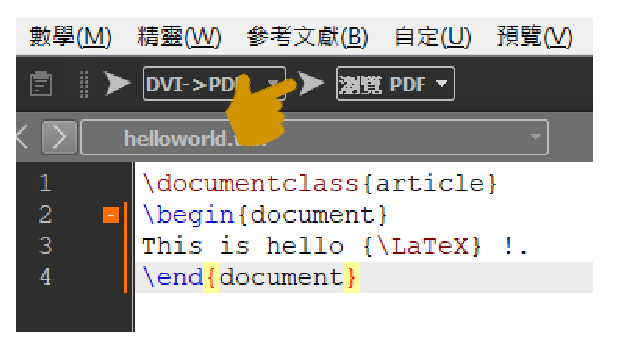
\includegraphics[width= 2.3in]{figs//s3}}
\caption{The basic procedure for LaTeX.}%
\label{fig.latex}%
\end{figure*}


\begin{figure*}[!t]
\centering
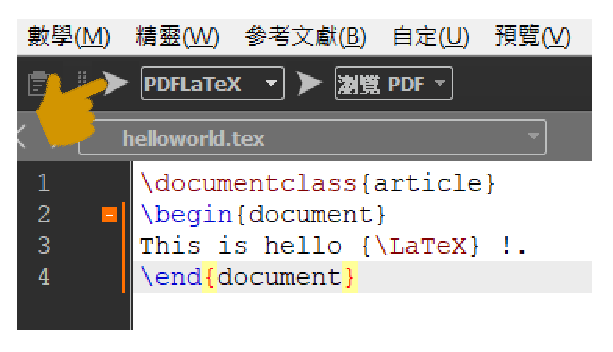
\includegraphics[width= 2.3in]{figs//s4}
\caption{The basic procedure for PDFLaTeX.}%
\label{fig.pdflatex}%
\end{figure*}



Now, go to this website (\url{https://www.sharelatex.com/learn}) to learn the basic knowledge of {\LaTeX}.

\section{Other resources}

\begin{itemize}
\item \url{https://en.wikibooks.org/wiki/LaTeX}
\item \url{https://tex.stackexchange.com/}
\end{itemize}


